% This is "sig-alternate.tex" V2.0 May 2012
% This file should be compiled with V2.5 of "sig-alternate.cls" May 2012
%
% This example file demonstrates the use of the 'sig-alternate.cls'
% V2.5 LaTeX2e document class file. It is for those submitting
% articles to ACM Conference Proceedings WHO DO NOT WISH TO
% STRICTLY ADHERE TO THE SIGS (PUBS-BOARD-ENDORSED) STYLE.
% The 'sig-alternate.cls' file will produce a similar-looking,
% albeit, 'tighter' paper resulting in, invariably, fewer pages.
%
% ----------------------------------------------------------------------------------------------------------------
% This .tex file (and associated .cls V2.5) produces:
%       1) The Permission Statement
%       2) The Conference (location) Info information
%       3) The Copyright Line with ACM data
%       4) NO page numbers
%
% as against the acm_proc_article-sp.cls file which
% DOES NOT produce 1) thru' 3) above.
%
% Using 'sig-alternate.cls' you have control, however, from within
% the source .tex file, over both the CopyrightYear
% (defaulted to 200X) and the ACM Copyright Data
% (defaulted to X-XXXXX-XX-X/XX/XX).
% e.g.
% \CopyrightYear{2007} will cause 2007 to appear in the copyright line.
% \crdata{0-12345-67-8/90/12} will cause 0-12345-67-8/90/12 to appear in the copyright line.
%
% ---------------------------------------------------------------------------------------------------------------
% This .tex source is an example which *does* use
% the .bib file (from which the .bbl file % is produced).
% REMEMBER HOWEVER: After having produced the .bbl file,
% and prior to final submission, you *NEED* to 'insert'
% your .bbl file into your source .tex file so as to provide
% ONE 'self-contained' source file.
%
%
% For tracking purposes - this is V2.0 - May 2012

\documentclass{sig-alternate}
\usepackage{color}
\usepackage[colorlinks,citecolor=blue]{hyperref}
\usepackage{listings}
\usepackage{xcolor}
\usepackage[danish]{babel}

\begin{document}

\conferenceinfo{Web Science}{2016 DIKU, Denmark}
\title{TEMPLATE\\WS 2016 Project 1}
\numberofauthors{1} 
\author{
\alignauthor 
Keep anonymous
}
\maketitle



%Write the introduction to the project here, in your own words. . 
\section{Introduction}
The scope of this project it to try and create a prediction model which, based on Google term history, can predict the real-life sales of vaccines. The terms are determined by short layman descriptions, and gathered by mining from Google Trends\footnote{\url{https://www.google.dk/trends/}}.

The following project was all done in python, using pre-made modules to assist in the mining and processing of trends.

In this project, the vaccines \textbf{PVC} \& \textbf{HPV} were examined. Any two vaccines should be fine, but I'm happy with these two, as their data differs in size, with PVC only creating 16 query items, while HPV has 65. Query items are also called Trends, and are described in the following section.

\section{Methodology}
\subsection{Trends}
In this project, trends are words which are commonly used when describing vaccines. Stopwords, which are words that only appear in text for grammatically reasons, do not count as trends. The trends are determined by reading multiple (in this case two) descriptions of a given vaccine, and then stripping each description of symbols and stopwords. Both descriptions are then compared to each other, and only words which occur in both descriptions qualify to be trends. This is a rather simple way of creating the trends, and some words, which only differ grammatically, such as \textit{alvorlig} and \textit {alvorlige} are considered different, even through they are functionally the same. However it proves sufficient for the scope of this project.
%Describe the methodology of this study in your own words. 

\subsection{Mining of Trends}
In order to mine the trends from Google, I resorted to using a python package called pytrends\footnote{\url{https://github.com/GeneralMills/pytrends}}, which provides for a simple framework for downloading .csv files from Google Trends. It works by signing into Google, and then, with different intervals, making a request after which it allows for download of the corresponding .csv file.

When downloading the .csv files, they can come with data in either a weekly or a monthly interval, most likely due to the popularity of certain terms, which prompts for more in-dept information. In order to accommodate for the difference of format, a simple python script was written, which would convert weekly data into monthly data, by making a crude estimation of a monthly value, based on average values and full week durations, which meant some weeks overlapped into the following month. A more advanced script should probably be written for a more precise estimation of monthly values, but for this project, I found the crude script to work well.

Certain trends may result in empty .csv files. For example, for PVC, \textit{vaccinen}, \textit{pneumokoksygdom} \& \textit{pneumokokvaccinen} came up empty, thus reducing the usable number of trends from 16 to 13.

 In these cases I simply skip the trend when doing further analysis.

\subsection{Prediction}
The choice of prediction method was randomly chosen to be that of Lasso. Lasso requires a Matrix, X, of dimensions $NxM$ where $N$ is the time frame we examine, here 57 months, and $M$ is the number of trends (13 and 61 after empty results have been removed). The provided data served as a ground truth  when preforming fitting of the model, and even through it holds data for 60 months, I only use the first 57, as to match the X Matrix.

Fitting of the model was done as part of a 5-fold cross-validation. The python package \textit{sklearn}\footnote{\url{http://scikit-learn.org/}} provided all the necessary tools for doing the splitting needed in the 5-fold cross-validation, as well as the model fitting and prediction.

\begin{lstlisting}[language=Python]
k_fold = cross_validation.KFold(len(X), 5)
\end{lstlisting}

would provide a \textit{k\_fold} consisting on five iterations on form $k, (train, test)$, where train is list of index values for training, and test is a smaller list for testing.

These values would allow me to gradually train the module, results of which are in the next section.

\newpage

\section{Findings}
First I examined PVC. Figure~\ref{fig:PVC} shows how my predictions for each of the five folds went.
\begin{figure}[h!]
\centering
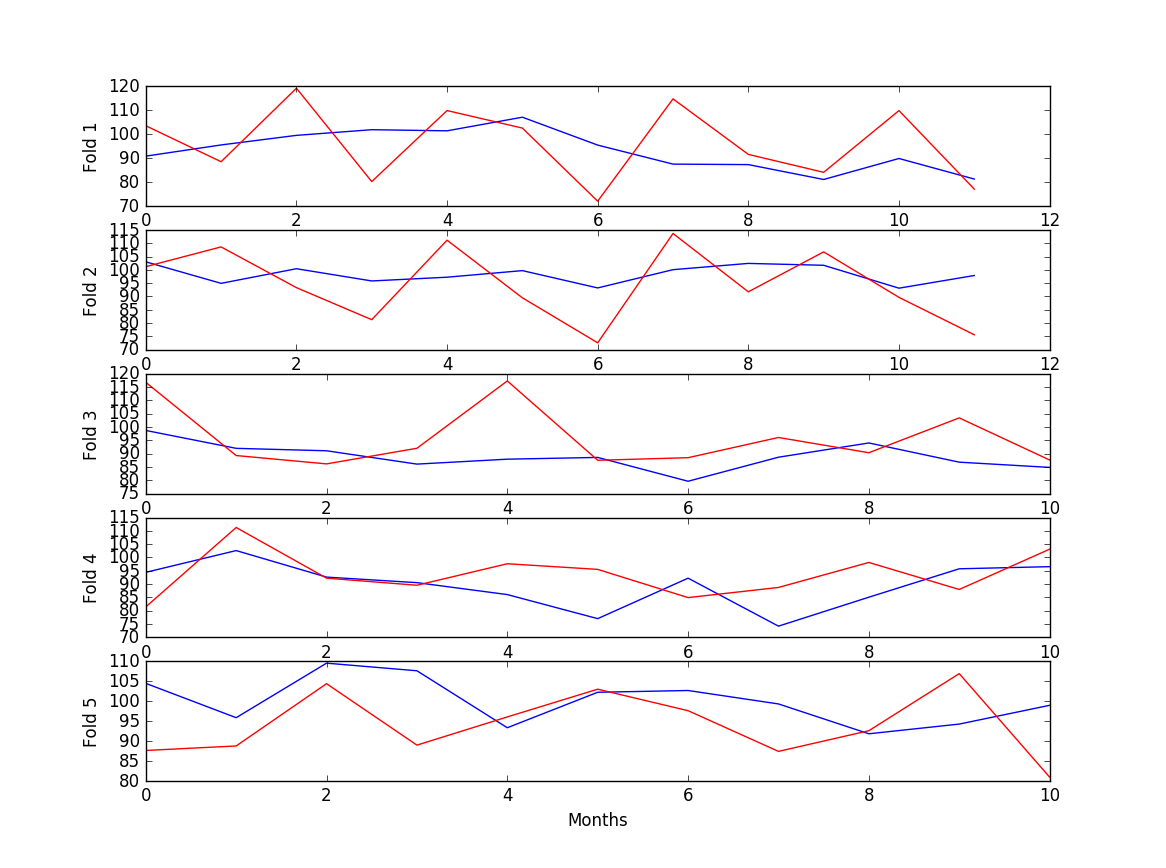
\includegraphics[width=0.5\textwidth]{PVC_Folds}
\caption{PVC predictions done in 5-fold cross-validation, red line is ground truth, blue is prediction.}
\label{fig:PVC}
\end{figure}
Looking at these 5 folds, the predictions being made, in \textcolor{blue}{blue}, does generally follow the provided data, in \textcolor{red}{red}, however not every fold is as spot on as fold 5. In figure~\ref{fig:HPV} the prediction are is spot on Fold 2, as it predicts the sudden drop at 6 months, and then it practically follows the curve from there.
\begin{figure}[h!]
\centering
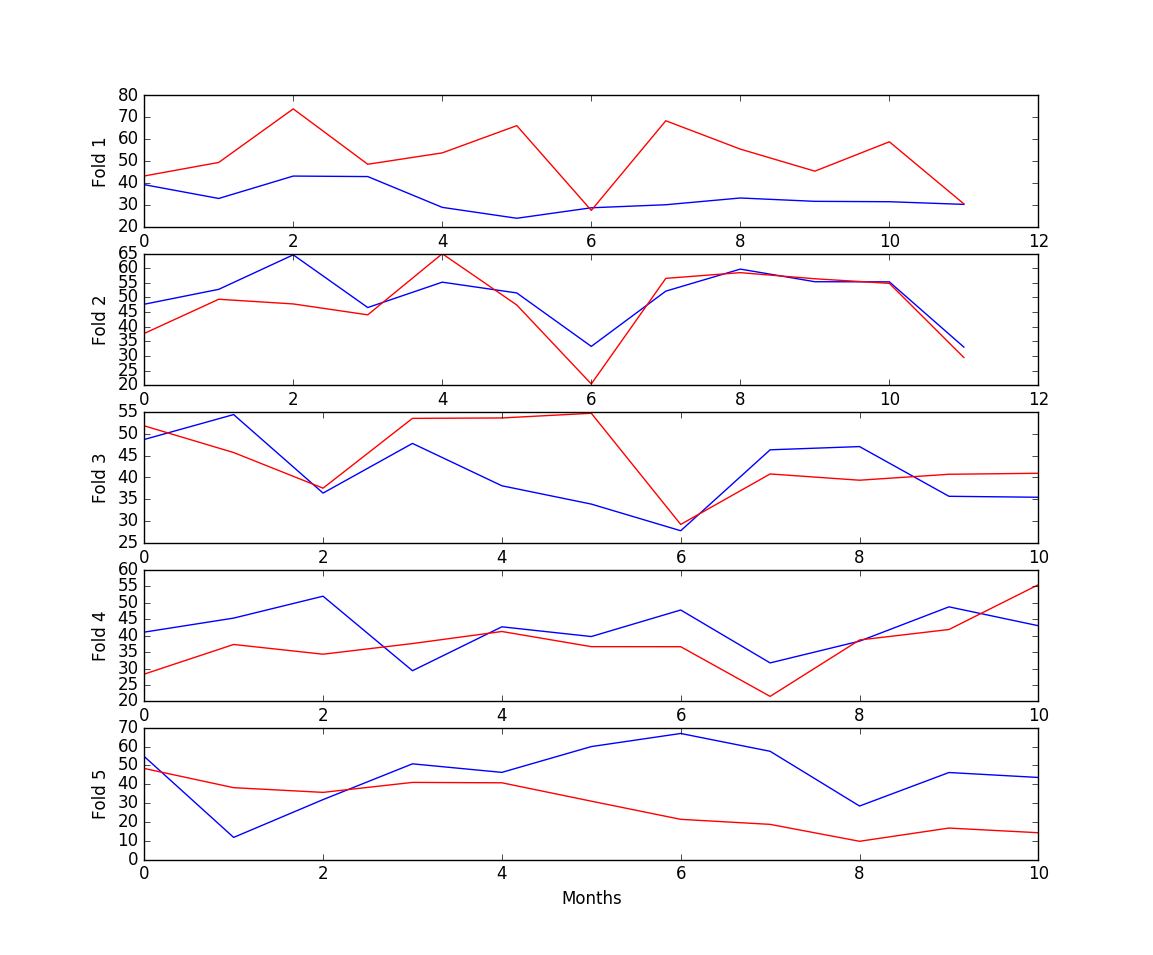
\includegraphics[width=0.5\textwidth]{HPV_Folds}
\caption{HPV predictions done in 5-fold cross-validation, red line is ground truth, blue is prediction.}
\label{fig:HPV}
\end{figure}

Other than simply looking at graphs, the way to determine how well a prediction model is doing, is by calculating the \textit{Root-mean-square error} (RMSE). In table~\ref{table:RMSE} I've provided the average RMSE over all five loops, for each vaccine, when looking at each of the provided clinical data files. Next to my results, I've entered the results which the original report\cite{H2016}, which this project was based on, was able to achieve.

For RMSE, the bigger the value you get, the worse your prediction probably is, and it's clear from the table, that my predictions were strictly worse than those provided in the original report.

\begin{table}[h!]
\centering
\caption{Lasso RMSE comparison, with Prediction Vaccination Uptake using Web Search Queries report.}
\begin{tabular}{|c|c|l|} \hline
& Original Report & My Findings \\ \hline
HPV-1 & 12.701 & 17.07 \\
HPV-2 & 18.423 &  23.202 \\
HPV-3 & 23.074 & 24.436 \\\hline
PCV-1 & 7.845 & 12.685 \\
PCV-2 & 9.770 & 14.448 \\
PCV-3 & 10.368 & 17.367\\
\hline\end{tabular}
\label{table:RMSE}
\end{table}

\section{Conclusions}
Examining table~\ref{table:RMSE} it's clear that my predictions did not preform as well as those in the original report. 
Especially not for HPV. I find the HPV to be interesting through, as the clinical data for the last 11 months are drastically lower than the previous 49 months, as plotted in figure~\ref{fig:HPV_FULL}
\begin{figure}[h!]
\centering
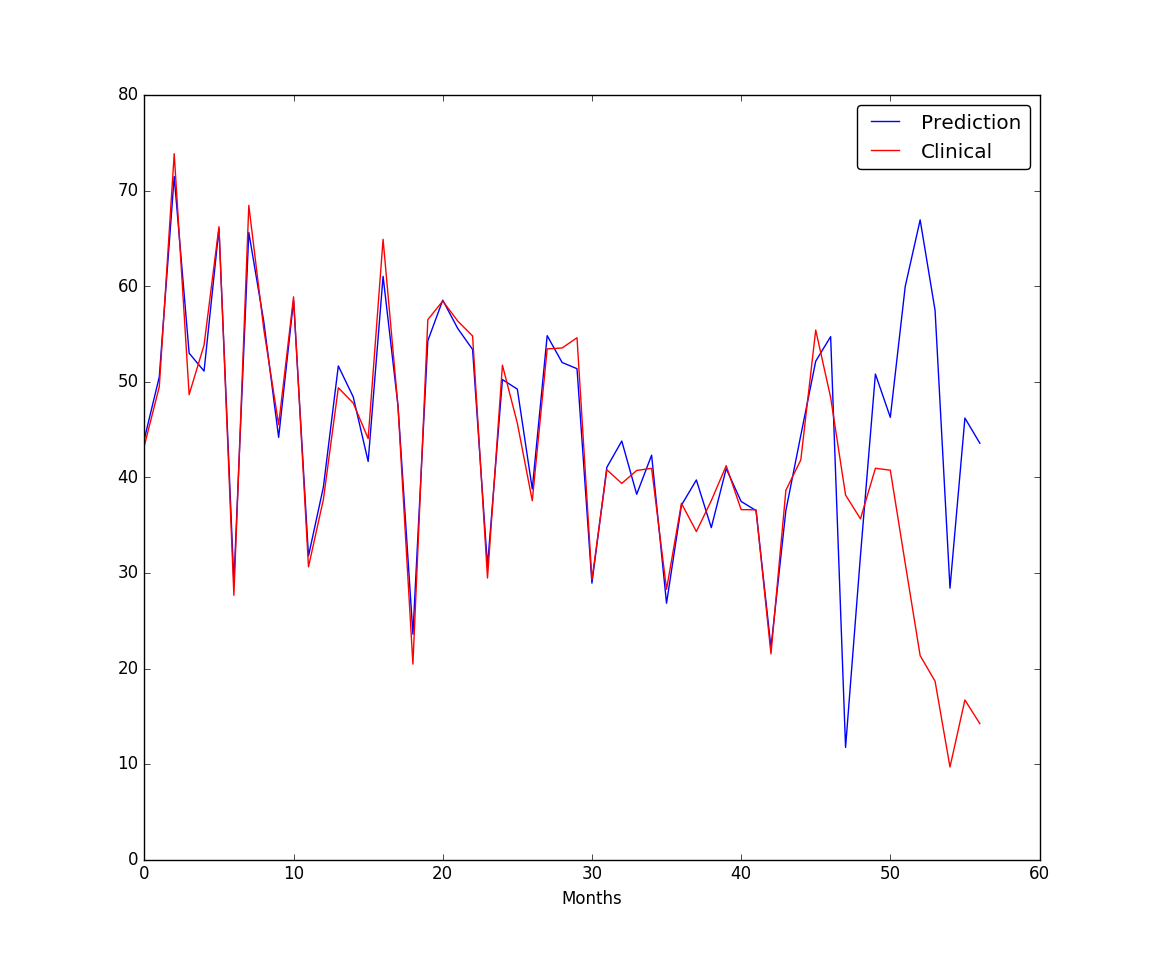
\includegraphics[width=0.5\textwidth]{hpv_full_prediction}
\caption{HPV Model predicted over full duration of data sample. red line is ground truth, blue is prediction.}
\label{fig:HPV_FULL}
\end{figure}
The model tries to predict a curve, as close to the previous 49 months, but since there's a sudden change, it fails to predict the vaccine frequency.

As for PVC, figure~\ref{fig:PVC_FULL}, the prediction is hard to compare to the clinical data. For each spike it predicts, it fair to say it misses one as well. This may be due to the, compared to the HPV vaccine, there's a limited amount of trends, 13 versus 61, and while the RMSE is not too far off, compared to the original paper, the actual usefulness of the current state of the predictions are very risky, should one try to invest based on these data point.
\begin{figure}[h!]
\centering
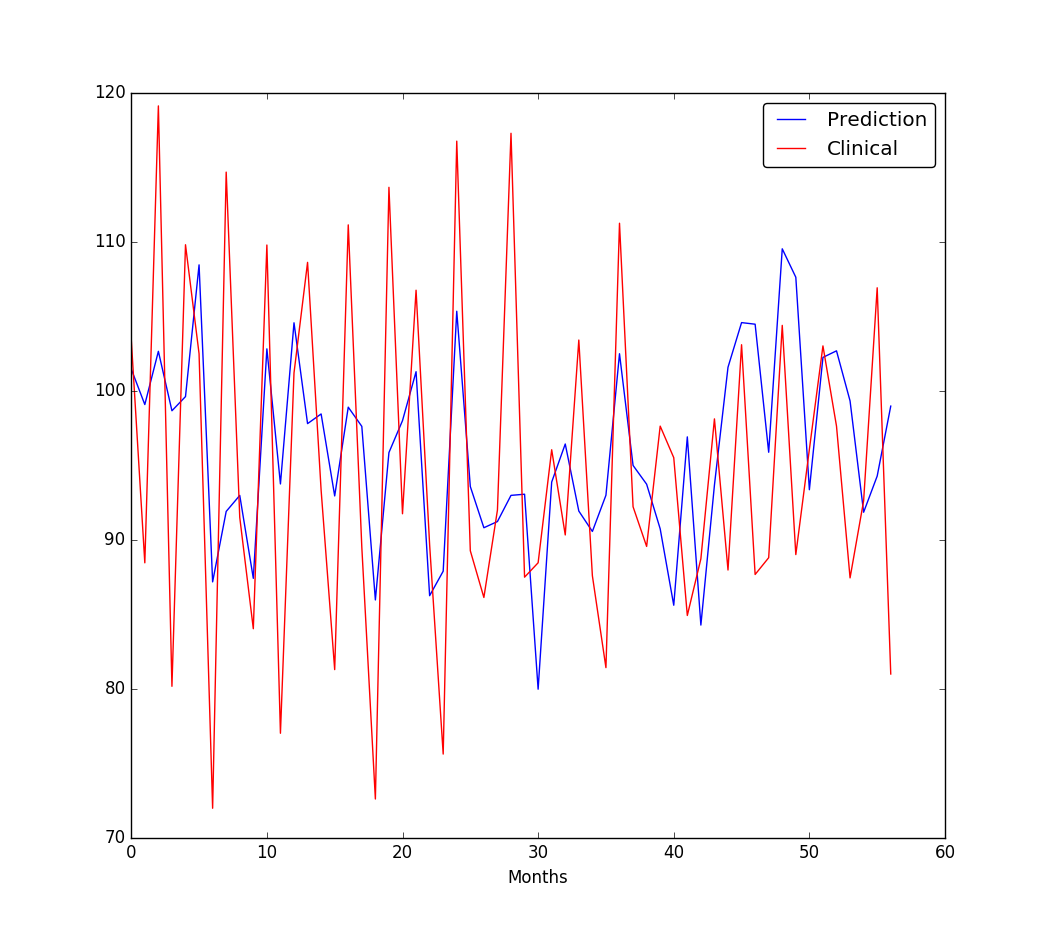
\includegraphics[width=0.5\textwidth]{pvc_full_prediction}
\caption{PVC Model predicted over full duration of data sample. red line is ground truth, blue is prediction.}
\label{fig:PVC_FULL}
\end{figure}

Overall, the exercise was engaging and a learning experience. But it's hard to be sure of the exact usefulness of the models as is.

% The following two commands are all you need in the
% initial runs of your .tex file to
% produce the bibliography for the citations in your paper.
\bibliographystyle{abbrv}
\bibliography{citations}  % sigproc.bib is the name of the Bibliography in this case
% You must have a proper ".bib" file
%  and remember to run:
% latex bibtex latex latex
% to resolve all references
%
% ACM needs 'a single self-contained file'!
%
%APPENDICES are optional
%\balancecolumns
%\appendix
%Appendix A
%\balancecolumns % GM June 2007
% That's all folks!
\end{document}
